\section{Background}

Quantum computing is a new framework of computation which promises exponential asymptotic speed-ups in certain problems compared to classical models by using quantum mechanical effects like \emph{superposition} and \emph{entanglement} to write fast algorithms which are also physically realizable. The de facto way of formally expressing universal quantum computation has traditionally been the quantum circuit model\cite{Nielsen2009}. This model uses unitary evolution for data encoding and processing while using hermitian measurements for recording computation results. Algorithms that are formulated for this model usually start with a qubit register initialized to a certain value, usually \(\ket0\). Then a unitary block, usually composed of smaller and reusable components called \emph{gates}, is applied to this register. Finally, the register is measured in \(\sigma_z\) basis and the outcome is written onto a classical register of the same size. This whole process is usually visualized through circuit diagrams. We provide a circuit diagram describing Grover's algorithm in Figure \ref{fig:grover} as a quantum circuit example.

\begin{figure}[htb]
  \centering
  \begin{quantikz}
  \lstick{\(\ket+^{\otimes n}\)} &\qwbundle{n}&\gate{U_\omega}  \gategroup[1,steps=4, style={dashed,inner xsep=6pt, xshift=4pt, inner ysep=18pt, yshift=8pt,fill=lightgray!8},background]{Grover Operator} & \gate{H}  \gategroup[1,steps=3, style={fill=lightgray!15},background]{Diffuser}& \gate{2\,\ket0\bra0 - I_n}  &  \gate{H} & [8pt] \ \ldots\ \qw & \meter{} & \cw  
\end{quantikz}
  \caption{Grover's Algorithm is composed of three steps. The initialization step creates an equal superposition of \(\ket0\) and \(\ket1\) for all the qubits in the input register. Then the unitary main body, the Grover Operator, is applied consecutively \(\approx\pi\sqrt{n}/4\) times. The last phase is the measurement of the input register.}\label{fig:grover}
\end{figure}

Quantum circuit model is certainly a quite popular, though not the only way of reasoning about quantum computation. Issues regarding its scalability led Russendorf et. al. to introduce the one-way quantum computer \cite{russendorf2001, russendorf2003}. At the heart of this model's mathematical foundations lie graph states. Graph states are considered by Hein et. al. as the results of a class of qubit interactions\cite{hein2006}. Within this formalism, qubits are described as vertices of a graph and the entanglement patterns between those qubits create the edges between those vertices. Since qubits can not self entangle, it should be possible to represent any graph state with a simple graph. 

Representation of graph states is an important matter. Even though they can be represented in terms of their wave functions, this turns out to be less than ideal. The wave function of an \(n\) qubit graph state has up to \(2^n\) terms, so it is in no way a compact representation. Furthermore, using the wave functions to represent graph states makes seeing entanglement patterns quite difficult. Due to these shortcomings of wave function representations, \emph{stabilizers}\cite{Nielsen2009} are used for representing graph states. The subgroup of \(n\) dimensional Pauli group \(\symcal{P}^n\) for which a graph state remains invariant with the application of its elements is called the stabilizer of that graph state. It's important to note that a graph state is uniquely represented by its stabilizer.

The main computational resource of a one-way quantum computer is a  \emph{cluster}, which is defined by Briegel and Russendorf as a \(d\)-dimensional rectangular lattice\cite{Briegel_2001} of qubits that have Ising-type interactions with their neighbours. The state of a cluster can be represented by a graph and can be prepared via application of controlled phase gates \(\sigma_z\) to vertices connected by an edge. Then, information is encoded and processed via a series of spin measurements to the cluster. Output of this process can then be accessed directly by a measurement of output qubits. An example execution of a one-way computer with a 2 dimensional cluster is given in Figure \ref{fig:cluster}. 

\begin{figure}
  \centering
  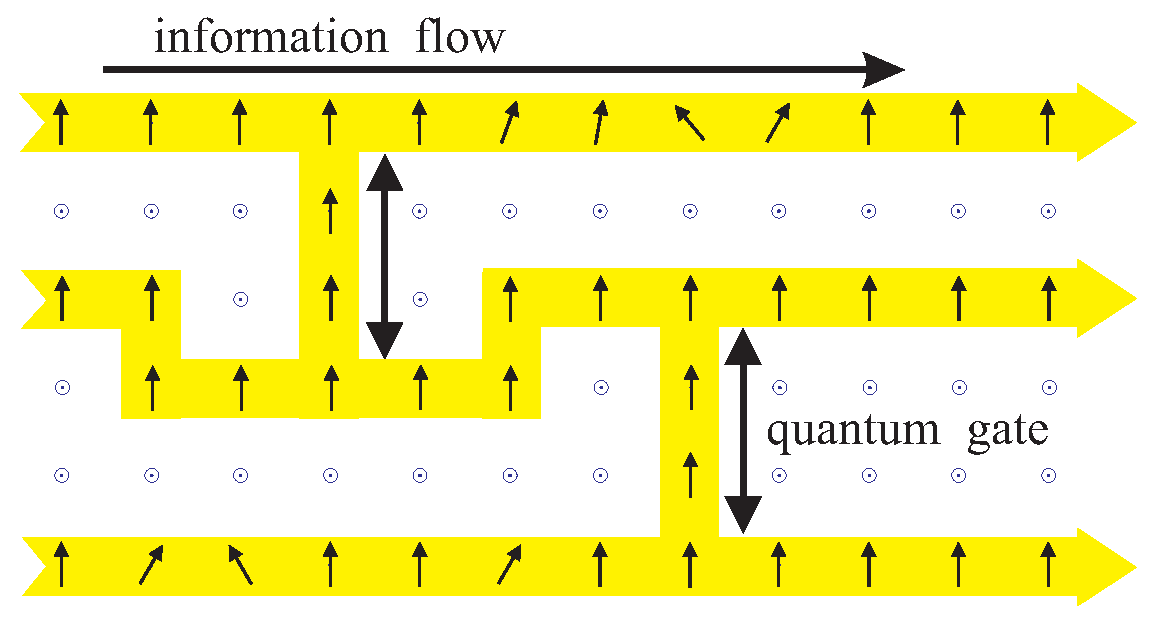
\includegraphics[
    width=0.75\textwidth
    ]{fig/figure1.eps}
  \caption{Computation on a cluster. \(\odot\) denotes a measurement along \(\sigma_z\), a vertical arrow denotes a measurement along \(\sigma_x\) and a tilted arrow denotes a measurement along \((\sigma_x + \sigma_y)/\sqrt2\). The image by Raussendorf et. al.\cite{russendorf2003} \label{fig:cluster}}
\end{figure}